\documentclass[fr]{../../../../../../eplexam}
\usepackage{tikz,siunitx}

\hypertitle{Compléments d'électricité}{5}{ELEC}{1755}{2018}{Janvier}
{Martin Braquet}
{Claude Oestges, Denis Flandre et Danielle Janvier}

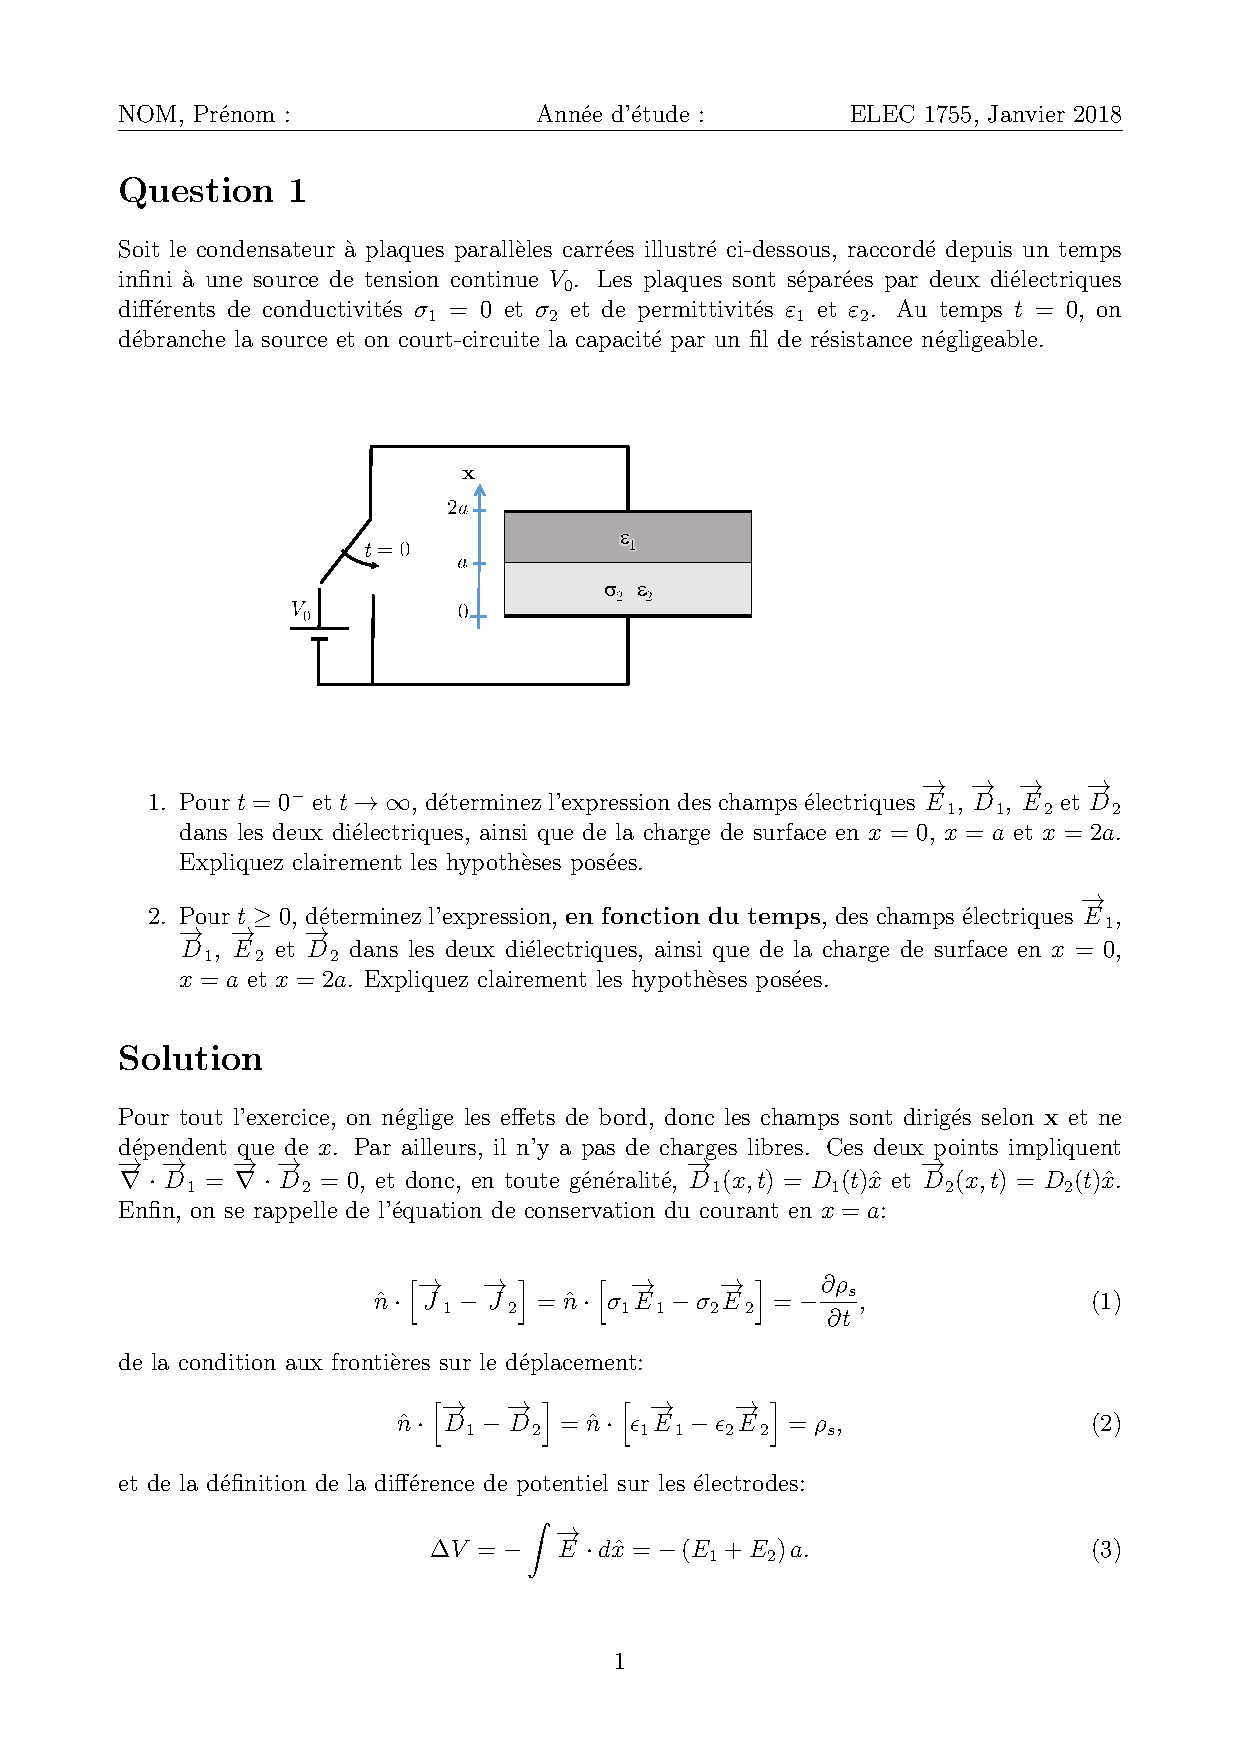
\includepdf[pages=-, scale=0.9, pagecommand={}]{examen_1755_janvier2018_Q1.pdf}

\setcounter{section}{1}
\section{Théorie de dispositifs}
Expliquer le principe de fonctionnement d'une diode, donner les graphes représentant
les variables intéressantes liées à ce dispositif.
\nosolution

\newpage 

\section{Exercice de dispositifs: FINFET}

La figure ci-dessous repréente un transitor MOSFET particulier: le FINFET.

\begin{center}
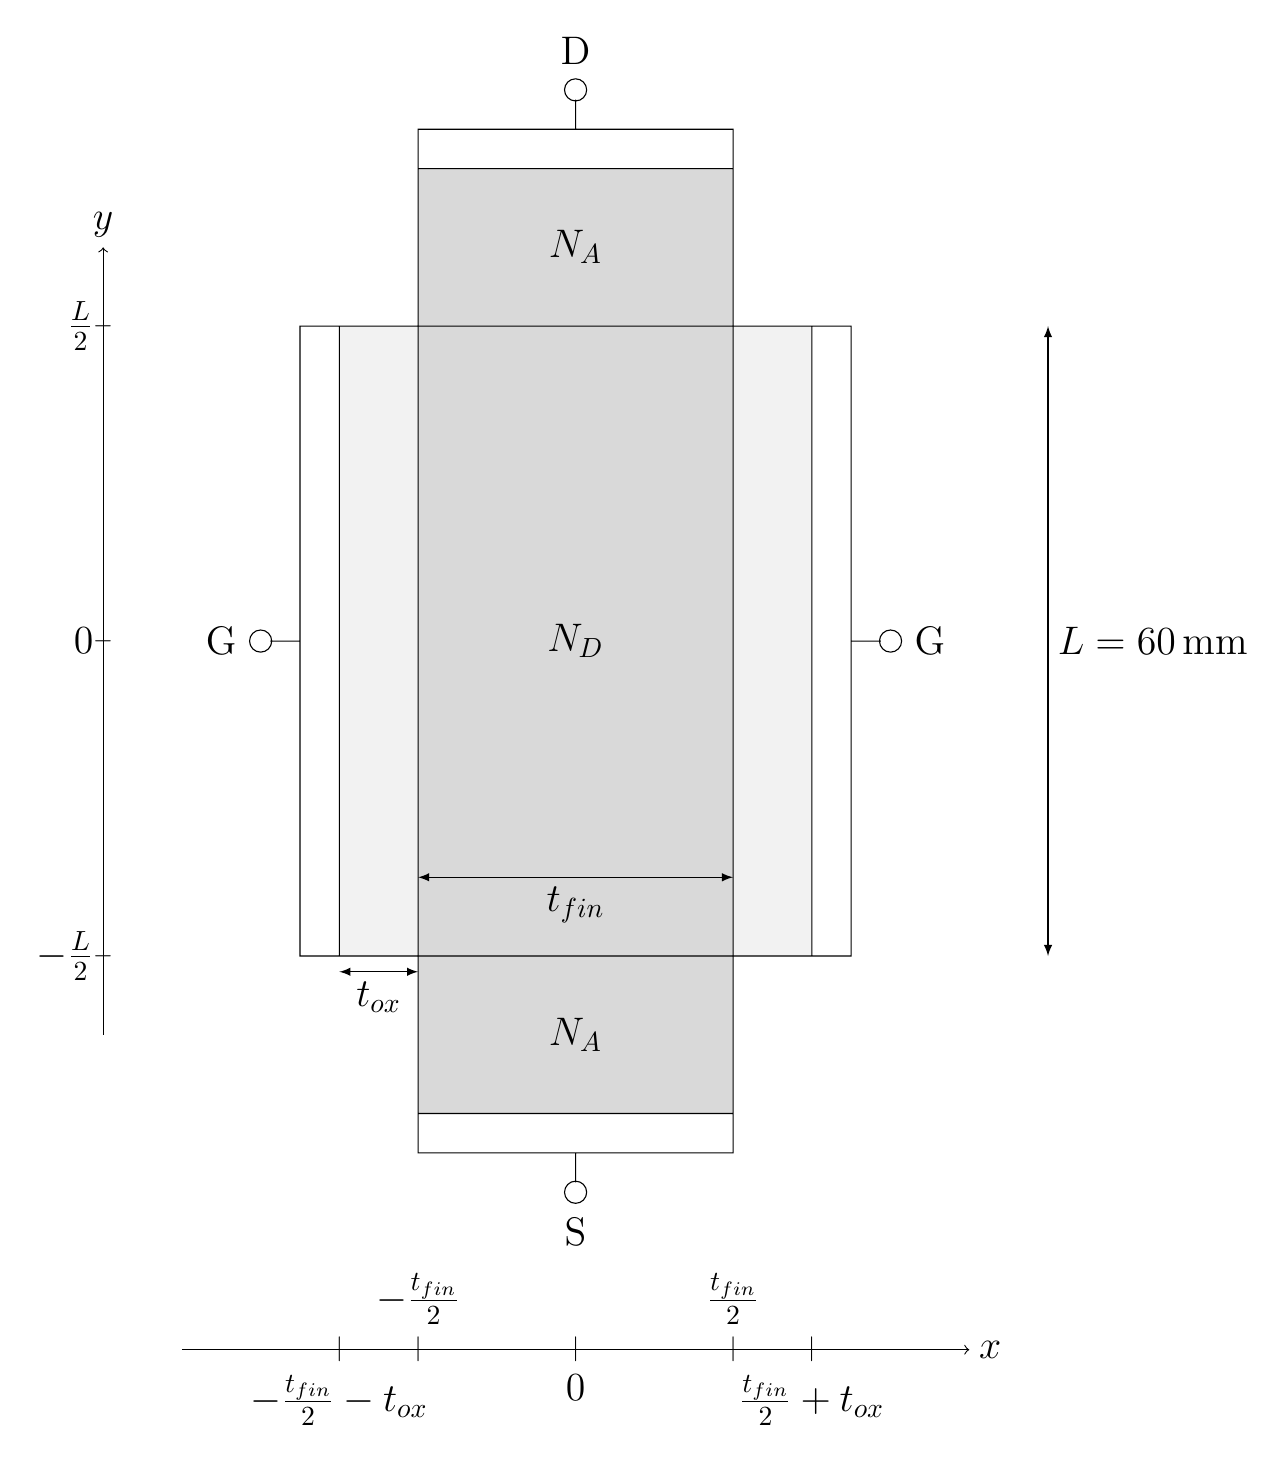
\begin{tikzpicture}
 \tikzstyle{every node}=[font=\Large]

 \fill[color=gray!10]
 (-3,-4) rectangle (-2,4)
 (2,-4) rectangle (3,4);
 \fill[color=gray!30]
 (-2,-6) rectangle (2,6);
 \draw
 (-3,-4) rectangle (3,4)
 (-2,-6) rectangle (2,6)
 (-2,-6.5) rectangle (2,-6)
 (-2,6.5) rectangle (2,6)
 (-2,-4) rectangle (2,4)
 (3,-4) rectangle (3.5,4)
 (-3.5,-4) rectangle (-3,4)
 (-2.5,-4.2) node [below] { $t_{ox}$}
 (0,-3) node [below] { $t_{fin}$}
 (0,-5) node { $N_A$}
 (0,5) node { $N_A$}
 (0,0) node { $N_D$}
 (-4,0) circle (4pt) node(c1) {}
 (-4.5,0) node { G}
 (-3.5,0) -- (c1.east)
 (4,0) circle (4pt) node(c2) {}
 (4.5,0) node { G}
 (3.5,0) -- (c2.west)
 (0,7) circle (4pt) node(c3) {}
 (0,7.5) node { D}
 (0,6.5) -- (c3.south)
 (0,-7) circle (4pt) node(c3) {}
 (0,-7.5) node { S}
 (0,-6.5) -- (c3.north)
 (-6,0) node {\small $-$}
 (-6,0) node[left] { 0}
 (-6,4) node {\small $-$}
 (-6,4) node[left] {$\frac{L}{2}$}
 (-6,-4) node {\small $-$}
 (-6,-4) node[left] {$-\frac{L}{2}$}
 (6,0) node[right] {$L=\SI{60}{mm}$}
 (-3,-9) node {\small $|$}
 (-3,-9) node[below,yshift=-0.2cm] {$-\frac{t_{fin}}{2}-t_{ox}$}
 (3,-9) node {\small $|$}
 (3,-9) node[below,yshift=-0.2cm] {$\frac{t_{fin}}{2}+t_{ox}$}
 (0,-9) node {\small $|$}
 (0,-9) node[below,yshift=-0.2cm] {0}
 (2,-9) node {\small $|$}
 (2,-9) node[above,yshift=0.2cm] {$\frac{t_{fin}}{2}$}
 (-2,-9) node {\small $|$}
 (-2,-9) node[above,yshift=0.2cm] {$-\frac{t_{fin}}{2}$}
 ;
 \draw[->] (-6,-5) -- (-6,5) node[above] {$y$};
 \draw[->] (-5,-9) -- (5,-9) node[right] {$x$};
 \draw [<->,>=latex] (-3,-4.2) -- (-2,-4.2);
 \draw [<->,>=latex] (2,-3) -- (-2,-3);
 \draw [<->,>=latex] (6,-4) -- (6,4);

\end{tikzpicture}
\end{center}

On considère que $\epsilon$ est constante et vaut \SI{e-10}{F/m}. La source est
connectée à la masse et il n'y a pas de charge dans l'oxyde de grille. On fait une analyse
unidimensionnelle selon $x$ en $y=0$. On a $N_d=\SI{e16}{cm^{-3}}$. Le FINFET a une double 
grille G. On considère que $t_{fin}=\SI{1}{\micro m}$, on ne peut donc pas parler d'un transistor FINFET avec une longueur pareille.

\begin{enumerate}
 \item S'agit-il d'un NMOS ou d'un PMOS? 
 \item Donner les différents modes de fonctionnement en fonction de $V_G$.
 \item Pour les questions suivantes, on considère le transistor en déplétion. Donner le graphe et l'expression de la densité de charge dans le dispositif.
 \item Avec l'équation de Poisson, donner le champ électrique et le potentiel en considérant
 pour la constante d'intégration que le potentiel est nul en $x=0$.
 \item On a $V_T=\SI{-0.8}{V}$, donner la profondeur maximale $x_{d,max}$ pour la zone de
 déplétion. Vérifier l'inégalité $t_{fin}>2x_{d,max}$ (si vous n'avez pas trouvé la valeur 
 de $x_{d,max}$, considérer que $x_{d,max}=\SI{280}{nm}$).
 \item Pour les questions suivantes, on considère le transistor en inversion. Donner le graphe et l'expression de la densité de charge dans le dispositif.
 \item On applique une tension $V_D$ telle que le transistor n'est pas en saturation, donner l'expression du courant
 et comparer avec le MOS classique.
 \item Pour les questions suivantes, on considère le transistor en inversion et $t_{fin}=\SI{400}{\micro m}$.
 Quel est l'impact du changement de longueur de $t_{fin}$ sur le régime de fonctionnement? Commment évolue la tension de sueil?
 \item Et si maintenant $t_{fin}=\SI{15}{\micro m}$, le transistor est un vrai FINFET. Que va-il se passer physiquement au niveau du canal?
 Quelles hypothèses supposées vraies dans les sous-questions précédentes n'est plus respectée?
 \end{enumerate}


\nosolution

\end{document}
